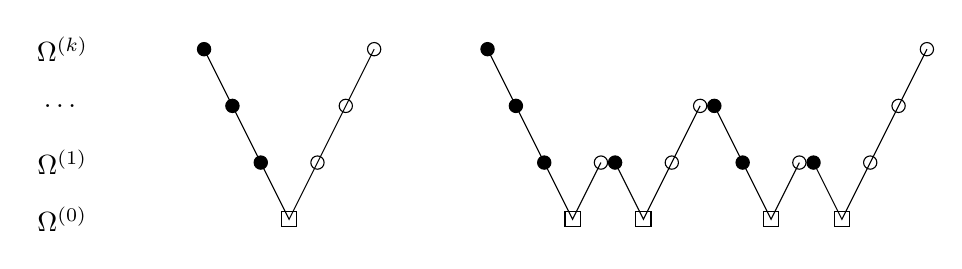
\begin{tikzpicture}[scale=1.2]
% see also fullcycle.tex

  \pgfmathsetmacro\hstep{0.3}
  \pgfmathsetmacro\vstep{0.6}
  \pgfmathsetmacro\ceps{0.08}   % size of square for coarse grid

% grid labels at left
  \node at (-1.5,3*\vstep) {$\Omega^{(k)}$};
  \node at (-1.5,2*\vstep) {\dots};
  \node at (-1.5,\vstep) {$\Omega^{(1)}$};
  \node at (-1.5,0.0) {$\Omega^{(0)}$};

% V-cycle
  \draw[black,thin] (0.0,3*\vstep) -- (\hstep,2*\vstep) --  (2*\hstep,\vstep) -- (3*\hstep,0.0)
                    -- (4*\hstep,\vstep) -- (5*\hstep,2*\vstep) -- (6*\hstep,3*\vstep);
  \filldraw (0.0,3*\vstep) circle (2.0pt);
  \filldraw (\hstep,2*\vstep) circle (2.0pt);
  \filldraw (2*\hstep,\vstep) circle (2.0pt);
  \draw     (3*\hstep-\ceps,-\ceps) rectangle (3*\hstep+\ceps,+\ceps);
  \draw     (4*\hstep,\vstep) circle (2.0pt);
  \draw     (5*\hstep,2*\vstep) circle (2.0pt);
  \draw     (6*\hstep,3*\vstep) circle (2.0pt);

% W-cycle
  \pgfmathsetmacro\woff{10*\hstep}
  \draw[shift={(\woff,0)},black,thin] (0.0,3*\vstep) -- (\hstep,2*\vstep) --  (2*\hstep,\vstep) -- (3*\hstep,0.0)
                    -- (4*\hstep,\vstep);
  \draw[shift={(\woff,0)},black,thin] (4.5*\hstep,\vstep) -- (5.5*\hstep,0.0) -- (6.5*\hstep,\vstep) --  (7.5*\hstep,2*\vstep);
  \draw[shift={(\woff,0)},black,thin] (8*\hstep,2*\vstep) -- (9*\hstep,\vstep) --  (10*\hstep,0.0) -- (11*\hstep,\vstep);
  \draw[shift={(\woff,0)},black,thin] (11.5*\hstep,\vstep) -- (12.5*\hstep,0.0) -- (13.5*\hstep,\vstep) -- (14.5*\hstep,2*\vstep) -- (15.5*\hstep,3*\vstep);
  \filldraw[shift={(\woff,0)}] (0.0,3*\vstep) circle (2.0pt);
  \filldraw[shift={(\woff,0)}] (\hstep,2*\vstep) circle (2.0pt);
  \filldraw[shift={(\woff,0)}] (2*\hstep,\vstep) circle (2.0pt);
  \draw[shift={(\woff,0)}]     (3*\hstep-\ceps,-\ceps) rectangle (3*\hstep+\ceps,+\ceps);
  \draw[shift={(\woff,0)}]     (4*\hstep,\vstep) circle (2.0pt);
  \filldraw[shift={(\woff,0)}] (4.5*\hstep,\vstep) circle (2.0pt);
  \draw[shift={(\woff,0)}]     (5.5*\hstep-\ceps,-\ceps) rectangle (5.5*\hstep+\ceps,+\ceps);
  \draw[shift={(\woff,0)}]     (6.5*\hstep,\vstep) circle (2.0pt);
  \draw[shift={(\woff,0)}]     (7.5*\hstep,2*\vstep) circle (2.0pt);
  \filldraw[shift={(\woff,0)}] (8.0*\hstep,2*\vstep) circle (2.0pt);
  \filldraw[shift={(\woff,0)}] (9.0*\hstep,\vstep) circle (2.0pt);
  \draw[shift={(\woff,0)}]     (10.0*\hstep-\ceps,-\ceps) rectangle (10.0*\hstep+\ceps,+\ceps);
  \draw[shift={(\woff,0)}]     (11.0*\hstep,\vstep) circle (2.0pt);
  \filldraw[shift={(\woff,0)}] (11.5*\hstep,\vstep) circle (2.0pt);
  \draw[shift={(\woff,0)}]     (12.5*\hstep-\ceps,-\ceps) rectangle (12.5*\hstep+\ceps,+\ceps);
  \draw[shift={(\woff,0)}]     (13.5*\hstep,\vstep) circle (2.0pt);
  \draw[shift={(\woff,0)}]     (14.5*\hstep,2*\vstep) circle (2.0pt);
  \draw[shift={(\woff,0)}]     (15.5*\hstep,3*\vstep) circle (2.0pt);

% option labels
  %\node at (3*\hstep,-0.6) {\texttt{-pc\_mg\_cycle\_type v}};
  %\node[shift={(\woff,0)}] at (9.3*\hstep,-0.6) {\texttt{-pc\_mg\_cycle\_type w}};

\end{tikzpicture}

